\chapter{Atmospheric Temperatures Variations}\label{ch:atm_variations}

The present chapter is devoted to the presentation of the numerical methods
and tools that has been adopted to calculate estimates of atmospsheric
brighness temperatures at our observation site. The CMB Atmospheric
Library, the software library that has been employed to perform
montecarlo simulations of the meteorological parameters and to solve the
radiative transfer equation, is introduced first. Then, our numerical
results, the seasonal matrices for atmospheric brightness
temperatures, are presented and discussed.

\section{The CMB Atmospheric Library}

The \emph{CMB Atmospheric Library}
(CAL)\footnote{\url{https://github.com/cmbgroundbased/cal}} is a free and
open source software library that has been developed to produce computer
simulations of atmospheric effects and telescope observations for
ground-based CMB experiments. CAL incorporates code extracted from the
well-known \emph{Time Ordered Astrophysics Scalable Tools} (TOAST) software
framework, making it and independent module, which can be exploited by
different CMB ground-based experiments. The CMB Atmospheric Library core is
written in \texttt{C++} programming language, in order to maintain high
performance.  However, \texttt{Python} programming language bindings are
provided to simplify its integration in experiments making use of
\texttt{Python} based pipelines.

CAL can be used to solve the atmospheric radiative transfer equation, which
has been discussed in \autoref{ss:radiative_transfer_eq}. To this end, the
library ships with
\emph{libaatm}\footnote{\url{https://github.com/hpc4cmb/libaatm}}, a
repackaged version of the \emph{Alma Atmospheric Transmission at Microwaves
Tools} (cit pardo), a model of the longwave atmospheric spectrum based on
broadband measurements and calculations. The model is fully applicable from
\SIrange{0}{2}{\tera\hertz} while including lines up to
\SI{10}{\tera\hertz}. Its primary goal is to simulate the
millimeter and submillimeter regions accessible from the ground.
libaatm discretize the atmosphere in a finite number of vertical
layers, from sea level to the tropopause, by a predefined internal profile.
Then, the radiative transfer equation is solved for each layer and
solutions are connected.

\subsection{CAL Relevant Methods}

The relevant methods which are provided by CAL and have been used in this
work follow:

\begin{itemize}
        \item \texttt{Weather}:

        This class can be initialized with the CDFs \texttt{.fits} file, which
        has been described in \autoref{s:CDF_fits_file}. It takes in input
        an UTC time structure with time resolution of \num{1} hour and
        returns pseudo-random realizations of meteorological parameters,
        determined by the probability distributions derived from the input
        \texttt{.fits} file.

        \item \texttt{atm\_atmospheric\_loading}:

        A wrapper function around libaatm methods. It solves the radiative
        transfer equation for a realization of the atmosphere defined by
        the values of $T_s$,
        $P_s$ and PWV, which are expected as input. It returns the value of sky
        brightness temperature in \si{\kelvin} (Rayleigh-Jeans) at a given
        frequency value, specified in input.

        \item \texttt{atm\_absorption\_coefficient}:

        As the latter one, this function solves the radiative transfer equation,
        but the total absorption coefficient,

        \begin{equation}
                \alpha_A\qty(\nu) = 1 - e^{-\tau_A\qty(\nu)}
        \end{equation}

        for the specified atmosphere realization at a given frequency is
        returned.
\end{itemize}

These three objects hides a significant implementation complexity, but are
simple in use. They can be jointly used to produce montecarlo simulations of
atmospheric brightness temperature at Pico del Teide, or at any other site
of interest.

%\section{The \texttt{tatmget} Computer Program}

\section{Atmospheric Temperatures Seasonal Matrices}

\begin{figure}
        \centering
        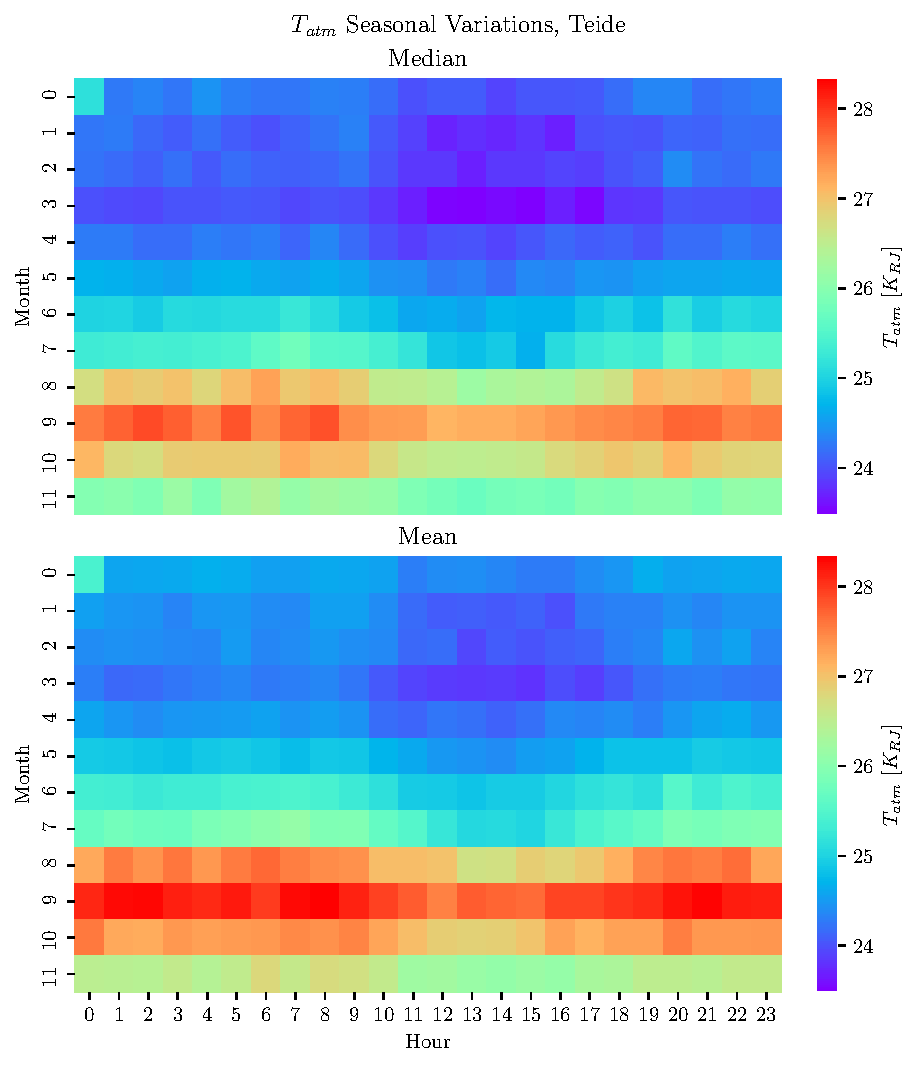
\includegraphics[width=\textwidth]{TATM_Matrices_nocal}
        \caption{$T_{atm}$ Seasonal Matrices}
        \label{fig:tatm_matrices_nocal}
\end{figure}

